\documentclass[onecolumn]{book}
\usepackage{fullpage}
\usepackage{yfonts}
\usepackage{palatcm}
%\usepackage{mathpazo}
\usepackage{amssymb}
\usepackage{amsmath}
\usepackage{amsthm}
\usepackage{eucal}
\usepackage{nicefrac}
\usepackage{graphics}
\usepackage{graphicx}
\usepackage{tabularx}
\usepackage{fancyvrb}
\usepackage[english]{babel}
\usepackage[small,bf,textfont=it,up,figurewithin=none]{caption}
\usepackage[indention=15pt]{subfig}
\usepackage{cite}
\usepackage[usenames,dvipsnames]{xcolor}
\usepackage{colortbl}
\usepackage{float}
\usepackage{multicol}
\usepackage{calc}
\usepackage{rotating}
\usepackage{afterpage}
\usepackage{verbatim}
\usepackage{longtable}
\usepackage{tablefootnote}
\usepackage[dotinlabels]{titletoc}
\usepackage[avantgarde]{quotchap}
\usepackage[square,comma,numbers]{natbib}
\usepackage{hyperref}
\hypersetup{colorlinks,linktocpage=true,citecolor=[rgb]{0,0.0,1.0},linkcolor=Red}
\usepackage{url}
\usepackage{booktabs}
\usepackage{fancybox}
\usepackage[framemethod=tikz]{mdframed}
\usetikzlibrary{shadows}
\usepackage[sectionbib]{chapterbib}
\usepackage{framed}
\usepackage{xcolor}
\usepackage{algpseudocode}
\usepackage{algorithm}
\usepackage{listings}
\lstset{numberbychapter=false}
\lstset{basicstyle=\ttfamily}
\usetikzlibrary{positioning,decorations.pathreplacing,fit}

\newcommand{\tikzmark}[2][]{%
  \tikz[remember picture,overlay,baseline=-.5ex] \node[#1] (#2) {};%
}

% \drawBrace[xshift]{beginningNode}{endingNode}
% This command draws a brace between two tikzmarks, to their right,
% no matter which one is the rightmost, and includes
% a node midway the brace, to write the comment.
% This command also creates a new node
% whose name is the concat of the names of beginning and ending nodes.
\newcommand*{\drawBrace}[4][0pt]{%
    \node[draw=none, fit={(#2) (#3)}, inner sep=0pt] (rectg) {};%
    \draw [decoration={brace,amplitude=0.3em},decorate,very thick,red]%
      ([xshift=#1]rectg.north east) --%
      coordinate[right=1em, midway] (#2#3)
      ([xshift=#1]rectg.south east);%
    \node[right=1.5em of #2#3] (#2#3-comment) {#4};
    \draw (#2#3-comment.west) edge (#2#3);
}%

\definecolor{red}{rgb}{1.0,0.0,0.0}
\definecolor{blue}{rgb}{0.0,0.0,1.0}
\definecolor{niceyellow}{rgb}{0.98,0.92,0.73}
\definecolor{niceyellow2}{rgb}{0.88,0.82,0.63}
\definecolor{nicegray}{rgb}{.753,.753,.753}
\definecolor{light-gray}{rgb}{.853,.853,.853}
\definecolor{light-blue}{rgb}{0.8,0.85,1}
\definecolor{emerald}{rgb}{0.19,0.5,0.38}
\definecolor{nicegreen}{rgb}{0.498,0.9,0.293}
\definecolor{olive-drab}{rgb}{0.42,0.55,0.137}
\definecolor{orange-red}{rgb}{1.0,0.27,0.0}

\newmdenv[shadow=true,shadowcolor=black,font=\sffamily,rightmargin=8pt]{shadedbox}

\newcommand{\dbar}{d\mkern-6mu\mathchar'26}


\arraycolsep 3pt
\tabcolsep 2pt
\arrayrulewidth .4pt
\doublerulesep 2pt
\fboxsep  = 3.0pt
\fboxrule = 0.4pt

\renewcommand{\topfraction}{0.95}
\renewcommand{\textfraction}{0.05}
%\renewcommand{\floatpagefraction}{0.95}

%\addtolength{\textheight}{17mm}
%\addtolength{\topmargin}{-7.5mm}

\renewcommand\floatpagefraction{0.1}

\begin{document}
\title{
\vskip -3.0cm
RASPA 3.0: Molecular Software Package for Adsorption and Diffusion in (Flexible) Nanoporous Materials
\vskip 0.25cm
\begin{figure}[H]
\centering
\includegraphics[width=10cm]{nu-110.jpg}
\end{figure}}
\author{
Youri Ran\\{email: y.a.ran@uva.nl}\\University of Amsterdam
\and
Shrinjay Sharma\\{email: S.Sharma-6@tudelft.nl}\\Delft University of Technology
\and
Salvador Rodr\'iguez G\'omez\\{email: salrodgom@upo.es}\\Universidad Pablo de Olavide
\and
Zhao Li\\{email: zhaoli2023@u.northwestern.edu}\\Northwestern University
\and
Sofia Calero\\{email: s.calero@tue.nl}\\Eindhoven University of Technology
\and
Thijs J.H. Vlugt\\{email: t.j.h.vlugt@tudelft.nl}\\Delft University of Technology
\and
Randall Q. Snurr\\{email: snurr@northwestern.edu}\\Northwestern University
\and
David Dubbeldam\\{email: d.dubbeldam@uva.nl}\\University of Amsterdam
}

\maketitle

\tableofcontents

\chapter{Introduction}


\section{Design philosophy}

\texttt{RASPA3} is a molecular simulation code for computing adsorption and diffusion in nanoporous materials, 
and thermodynamic and transport properties of fluids. 
It implements force field based classical Monte Carlo/Molecular Dynamics in various ensembles.
\texttt{RASPA3} can be used for the simulation of molecules in gases, fluids, zeolites, aluminosilicates,
metal-organic frameworks, and carbon nanotubes.
One of the main applications of \texttt{RASPA3} is to compute adsorption isotherms and to 
understand the atomic-level mechanism of adsorption and separations.


\texttt{RASPA3} is redesigned and rewritten from the ground up in \texttt{C++23}, based on the following ideas:
\begin{itemize}
  \item{Composition and value semantics}\\
    Major improvements in efficiency result from the implementation of \texttt{C++} code based on composition 
  and value semantics (in contrast to inheritance and reference semantics). Composition is a structural 
  approach in which complex objects are built from simple building blocks. Value semantics avoid 
  sharing mutable state and upholds the independence of values to support local reasoning. 
  References are only used implicitly,  at function boundaries, and are never stored. 
  This style of coding has many advantages. Avoiding complex inheritance hierarchies and reducing the 
  need for virtual functions lead to major code simplifications. It encourages code clarity and 
  local reasoning. With composition, components are directly included in an object, removing the 
  necessity for pointers, manual memory allocations, and indirections. This leads to straightforward 
  memory patterns and access safety. Lifetimes of objects are coupled with composition, eliminating the 
  need for explicit memory management. These lead to better compiler optimization and therefore performance of the code.
  \item{Correctness and accuracy}\\
    For all the techniques and algorithms available in \texttt{RASPA3} we have implemented the 'best' ones available in literature. 
    For example, \texttt{RASPA3} uses Configurational-Bias Monte-Carlo, it uses the Ewald summation for electrostatics,
  molecular dynamics is based on 'symplectic' integrators, all Monte-Carlo moves obey detailed balance etc.
  Unit tests test the smallest functional units of code and prevent developers breaking existing code when 
  refactoring or adding new code.
    The unit tests in \texttt{RASPA3} are arranged hierarchically. Atoms are placed at several distances and the 
  Lennard-Jones potentials are tested and compared with the analytically computed energy. 
  Then molecules are placed within a zeolite framework at predetermined positions and compared to the 
    energies computed with \texttt{RASPA2}.
  The various energy routines used in biased-sampling are tested by comparing to the general routines.
  The various routines for the gradients are tested by comparing the computed gradients to the values 
  computed by finite difference schemes based on the energy. Likewise, the strain-derivative tensor 
  (related to the pressure) is tested by comparing to the values computed by finite difference schemes 
  based on the energy of a strained cell.
  \item{Input made easy}\\
    The input of \texttt{RASPA3} has been changed to \texttt{JSON} format. 
    \texttt{JSON} stands for \texttt{JavaScript Object Notation}. It is a lightweight data-interchange format in plain text 
  written in JavaScript object notation. It is language independent.
  The requirements for the input files is kept as minimal as possible. 
  Only for more advanced options extra commands in the input file are
  needed. Also the format of the input is straightforward. Default settings are usually the best ones. 
  Fugacity coefficients and excess adsorption are automatically computed.
  \item{Output made easy}\\
    Similarly, the \texttt{JSON} format is now also used for the output. Where previously all initial data 
    (e.g. hardware info, unit conversion factors) and statistics (e.g. \texttt{CPU} timings, \texttt{MC} move statistics) 
    were written to a text file, these are now written as a nested dictionary to a \texttt{JSON} file.
  \item{Integrated simulation environment}\\
    The \texttt{RASPA3} \texttt{C++} simulation engine is made available to \texttt{Python} via a \texttt{Pybind11} interface. 
    For use in \texttt{Python}, \texttt{RASPA3} is built as a shared library, allowing its functions to be used by \texttt{Python}
  users and enabling seamless interactions with the simulation routines.
    Through the API, the library allows for invocation of \texttt{RASPA3}'s simulation routines from \texttt{Python} scripts, 
    calling the same simulation routines as via the \texttt{JSON} input. This execution directly from \texttt{Python} enables 
    the ability to prototype simulation settings and incorporate \texttt{RASPA3} into existing workflows.
  Extension and modification of the code is relatively straightforward.
\end{itemize}

\section{Units and conventions}
\begin{itemize}
  \item{The standard units in \texttt{RASPA} from which all other units are derived are:}\\
\vskip 0.1cm
\begin{tabularx}{\linewidth}{l|l|l|l}
 quantity & symbol & unit & value\\
\hline
 length      & $l$    & \AA ngstrom   & $10^{-10}$ m\\
 temperature & $T$    & Kelvin        & K\\
 mass        & $m$    & atomic mass   & $1.6605402\times 10^{-27}$ kg\\
 time        & $t$    & pico seconds  & $10^{-12}$ s\\
 charge      & $q$    & atomic charge & $1.60217733\times 10^{-19}$ C/particle\\
\hline
\end{tabularx}
\vskip 0.1cm

\noindent Some examples of derived units:\\

\begin{tabularx}{\linewidth}{l|l|l|l}
 quantity & symbol & units & conversion value\\
\hline
 energy             & $U$    & $J=\text{mass}\times\text{length}^2/\text{time}^2$ & $1.66054\times10^{-23}$ (=10 J/mol)\\
 pressure           & $p$    & $\text{Pa}=\text{mass}/(\text{length}\times\text{time}^2)$  & $1.66054\times10^7$\\
 diffusion constant & $D$    & $D=\text{length}^2/\text{time}$ & $1\times10^{-8}$\\
 force              & $f$    & $f=\text{length}/\text{time}^2$ & $1.66054\times 10^{-13}$\\
 \dots              & \dots  & \dots                                & \dots \\
\hline
\end{tabularx}\\

A pressure input of 10 Pascal in the input file, is converted to 'internal units' by dividing by $1.66054\times10^7$. In the
output any internal pressure is printed, multiplied by $1.66054\times10^7$. It is not necessary to convert units besides
input and output, with a few exceptions. One of them is the Coulombic conversion factor
\begin{equation}
  \frac{q_i q_j}{4\pi \epsilon_0}=\frac{\text{charge}^2}{4 \pi \times \text{electric constant}\times\text{length}\times\text{energy}}=138935.4834964017
\end{equation}
with the electric constant as $8.8541878176\times10^{-12}$ in units of $\text{C}^2/(\text{N}.\text{m}^2)$. This factor is needed to convert the
electrostatic energy to the internal units at every evaluation. 

\noindent
The Boltzmann's constant $k_B$ is
\begin{equation}
 k_B=\text{Boltzmann constant}/\text{energy}=0.8314464919
\end{equation}
with the Boltzmann constant as $1.380650324\times10^{-23}$ in units of J/K, and $k_B=0.8314464919$ in internal units.

\item{Numbering is based on the \texttt{C}-convention, i.e. starting from zero.}
\item{Files in the current directory always have preference.}\\
Sometimes one would like to try various parameters for force field fitting for example. In order to avoid
making a lot of directories for each force field it is more convenient to have the 
'\texttt{force\_field.def}' file in the \emph{current} directory.
\end{itemize}

\section{Compiling and installing \texttt{RASPA}}

\subsection{Requirements}

\texttt{CMake 3.28} and later support \texttt{C++} modules. 
\texttt{C++20} named modules are now supported by the \texttt{Ninja Generator 1.11} or newer in combination 
with the \texttt{LLVM/Clang 16.0} and newer, \texttt{MSVC toolset 14.34} and newer, or \texttt{GCC 14} and newer. 
We recommend LLVM/Clang 18 or higher for compiling \texttt{RASPA3}. This version has support 
for \verb+std::format+, \verb+std::print+, and \verb+std::jthread+. 
The output-files of \texttt{RASPA3} are in \texttt{UTF-8} encoding and contain unicode characters (e.g. for \AA).
\texttt{RASPA3} depends on
\begin{itemize}
  \item{\texttt{C++23} compliant compiler}
  \item{\texttt{Cmake 3.28}}
  \item{\texttt{Ninja Generator 1.11}}
  \item{\texttt{Openmp}}
  \item{\texttt{hdf5}}
  \item{\texttt{lapack} and \texttt{blas} (64-bit integers)}
  \item{\texttt{pybind11}}
\end{itemize}

\subsection{\texttt{RASPA} from '\texttt{git}'}

Working with '\texttt{git}' and a remote repository  means that you will have to distinguish between two locations of the code:
\begin{enumerate}
 \item{The repository (visible to everyone)}
 \item{your local copy (only visible to you)}
\end{enumerate}

To check-out the code for the first time do:
\begin{verbatim}
     git clone https://github.com/iraspa/RASPA3
\end{verbatim}
After that, you can update the code by using
\begin{verbatim}
     git pull
\end{verbatim}

\subsection{Installing \texttt{RASPA}}

Download one of the precompiled packages from
\begin{framed}
  \begin{quote}
    \url{https://github.com/iRASPA/RASPA3/releases}
  \end{quote}
\end{framed}
In Figure \ref{fig: binary_packages} one can find the list of packages. 
These include packages for \texttt{macOS} (both \texttt{intel} and \texttt{apple silicon}),
windows (both \texttt{intel} en \texttt{arm64}) and many \texttt{Linux} distributions.

\begin{figure}[p]
 \centering
  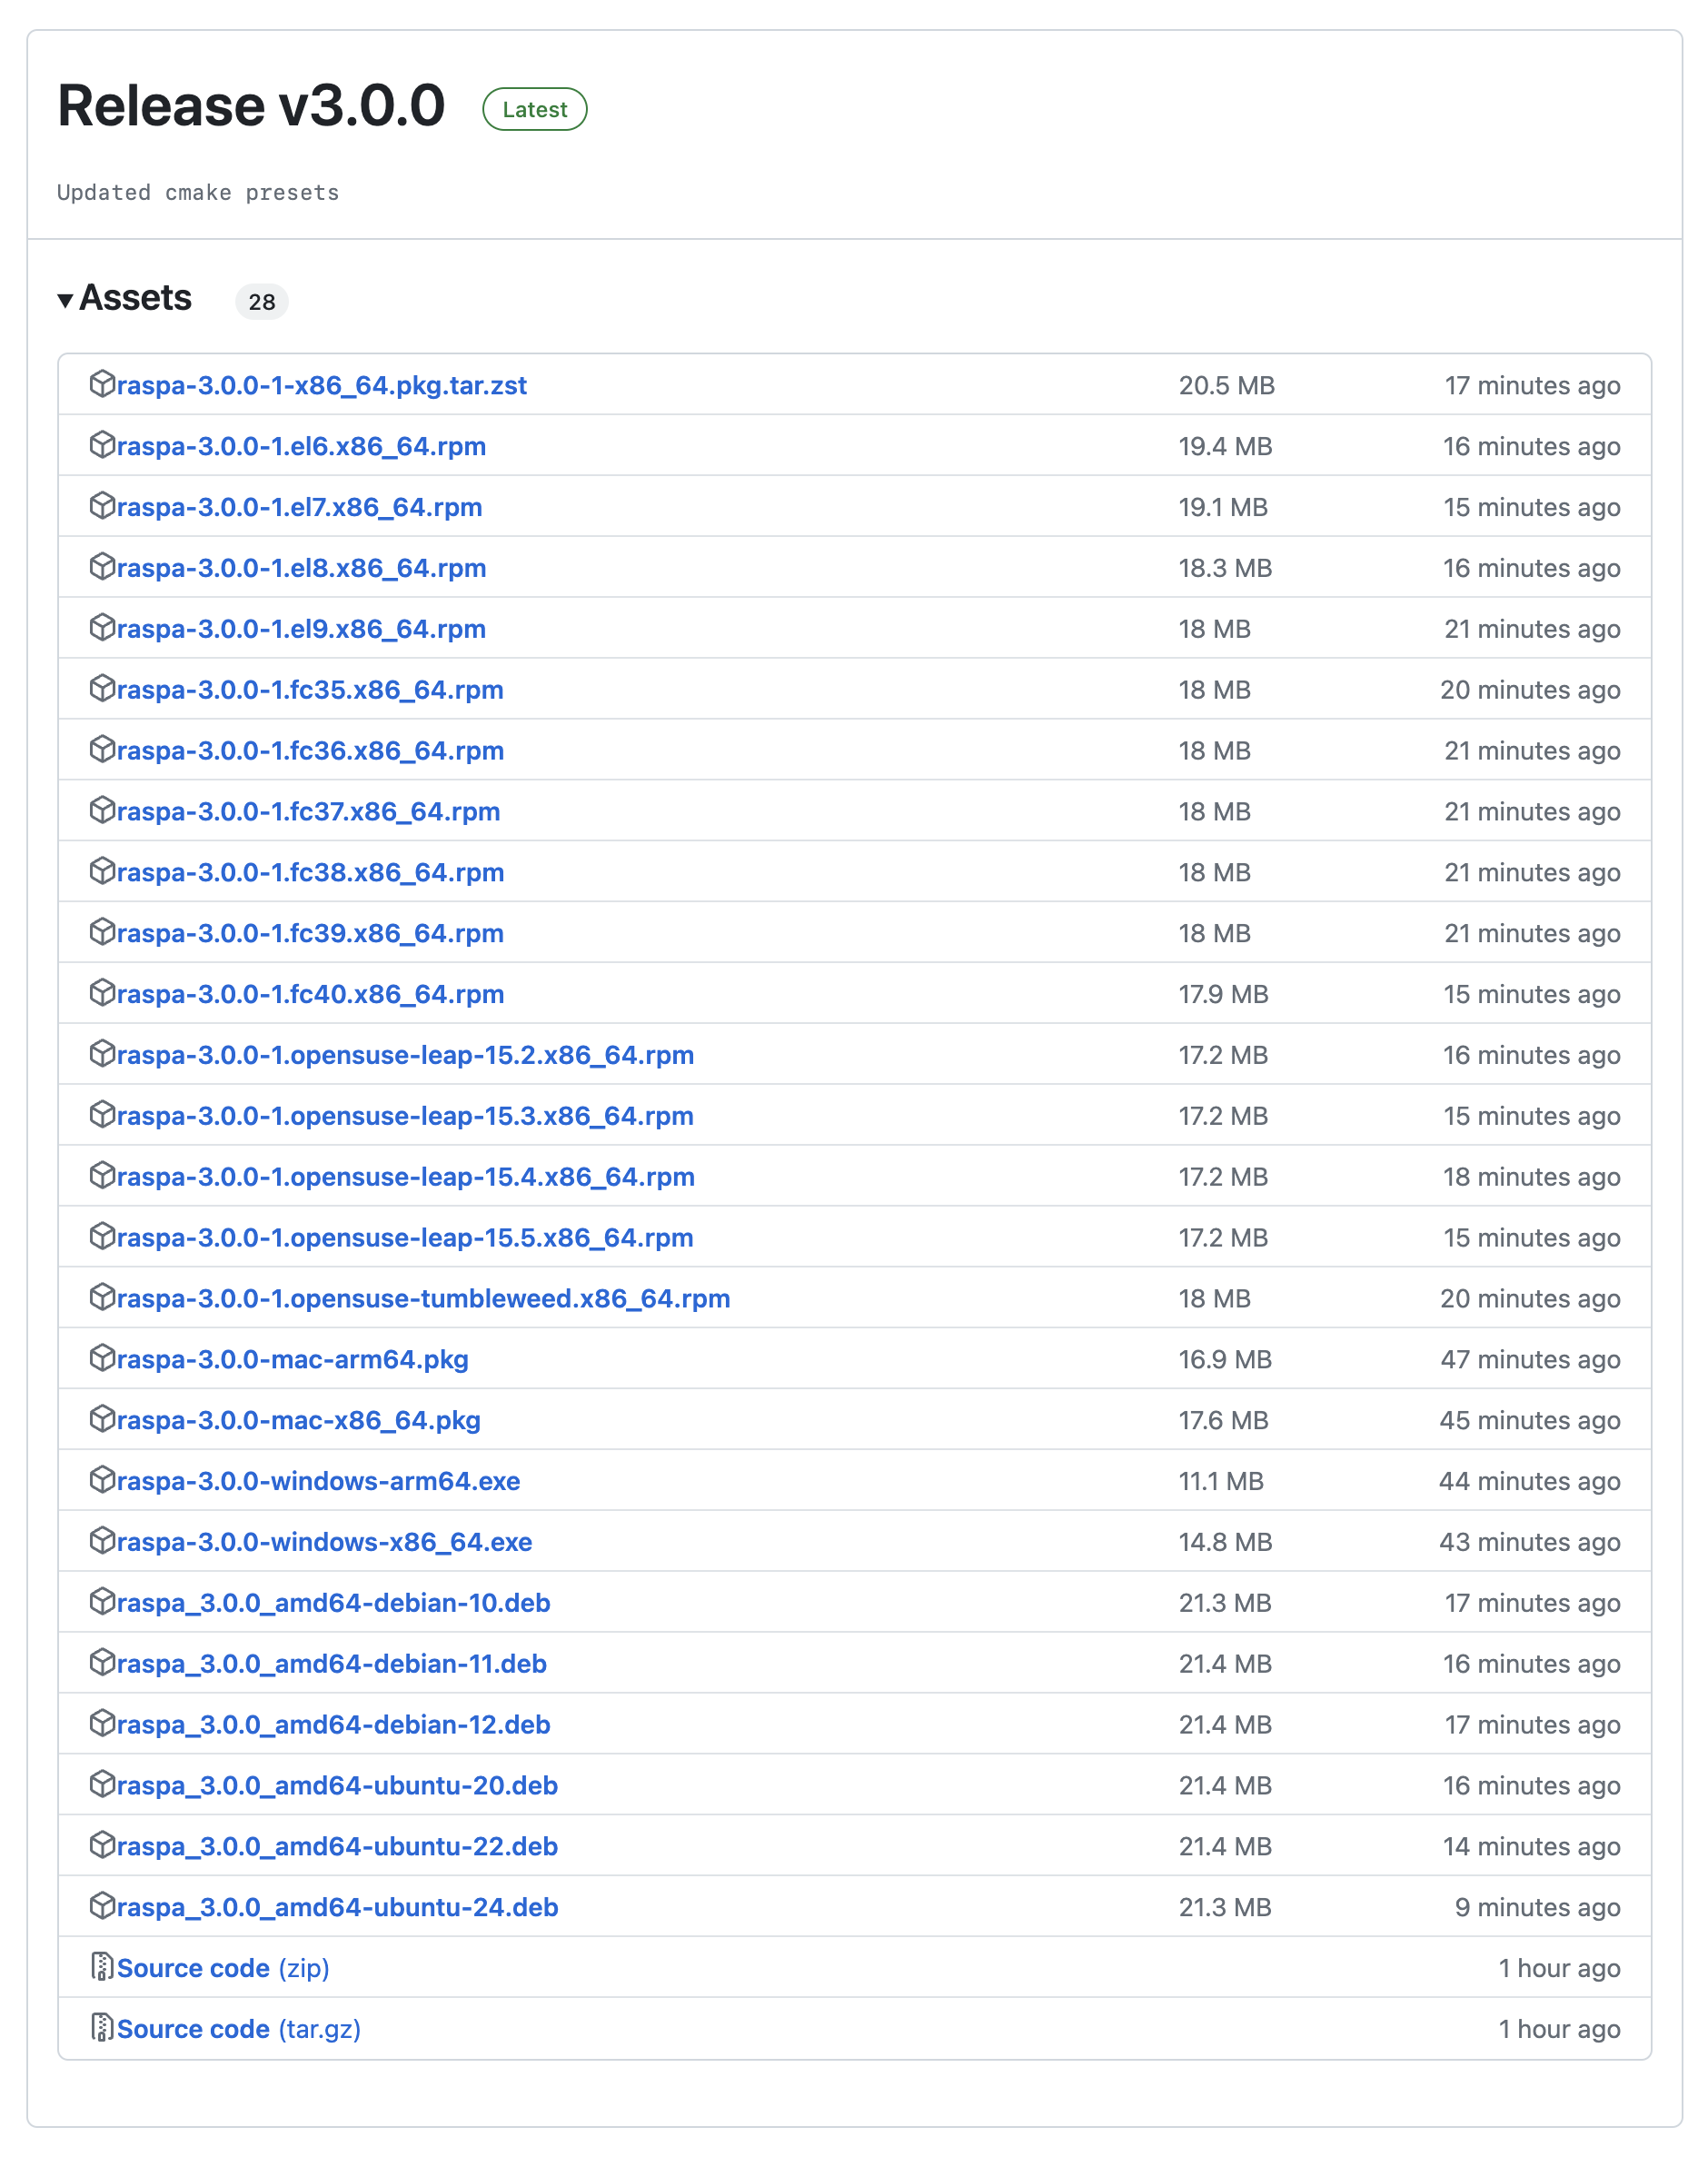
\includegraphics[width=0.95\linewidth]{introduction/raspa3_releases.png}
  \caption{List of available binary packages: \texttt{Linux} distributions based on \texttt{Red Hat} and 
  \texttt{OpenSUSE} (\texttt{rpm}-packages), \texttt{Debian} (\texttt{deb}-packages), and \texttt{Arch} \texttt{Linux} 
  (\texttt{tar.zst} packages), installers for \texttt{intel}- and \texttt{apple-silicon} macs,
  and installers for \texttt{intel}- and \texttt{arm64-Windows} computers.}
  \label{fig: binary_packages}
\end{figure}
\begin{table}[p]
  \scriptsize
  \begin{tabularx}{\linewidth}{X}
    \multicolumn{1}{c}{\texttt{Archlinux}}\\
    \hline
      \verb+pacman -Sy\verb+\\
      \verb+pacman -S wget\verb+\\
      \verb+wget https://github.com/iRASPA/RASPA3/releases/download/v3.0.0/raspa-3.0.0-1-x86_64.pkg.tar.zst+ \\
      \verb+pacman -U ./raspa-3.0.0-1-x86_64.pkg.tar.zst+\\
  \end{tabularx}
  \newline
\vspace*{0.5 cm}
\newline
  \begin{tabularx}{\linewidth}{c|X}
    \multicolumn{2}{c}{\texttt{Redhat}}\\
   \hline
  9 & \verb+yum install https://github.com/iRASPA/RASPA3/releases/download/v3.0.0/raspa-3.0.0-1.el9.x86_64.rpm+\\
     \hline
  8 & \verb+yum install https://github.com/iRASPA/RASPA3/releases/download/v3.0.0/raspa-3.0.0-1.el8.x86_64.rpm+\\
     \hline
  7 & \verb+yum install https://github.com/iRASPA/RASPA3/releases/download/v3.0.0/raspa-3.0.0-1.el7.x86_64.rpm+\\
     \hline
  6 & \verb+yum install https://github.com/iRASPA/RASPA3/releases/download/v3.0.0/raspa-3.0.0-1.el6.x86_64.rpm+\\
  \end{tabularx}
  \newline
\vspace*{0.5 cm}
\newline
  \begin{tabularx}{\linewidth}{c|X}
    \multicolumn{2}{c}{\texttt{Fedora}}\\
   \hline
  40 & \verb+dnf install https://github.com/iRASPA/RASPA3/releases/download/v3.0.0/raspa-3.0.0-1.fc40.x86_64.rpm+\\
     \hline
  39 & \verb+dnf install https://github.com/iRASPA/RASPA3/releases/download/v3.0.0/raspa-3.0.0-1.fc39.x86_64.rpm+\\
     \hline
  38 & \verb+dnf install https://github.com/iRASPA/RASPA3/releases/download/v3.0.0/raspa-3.0.0-1.fc38.x86_64.rpm+\\
     \hline
  37 & \verb+dnf install https://github.com/iRASPA/RASPA3/releases/download/v3.0.0/raspa-3.0.0-1.fc37.x86_64.rpm+\\
     \hline
  36 & \verb+dnf install https://github.com/iRASPA/RASPA3/releases/download/v3.0.0/raspa-3.0.0-1.fc36.x86_64.rpm+\\
     \hline
  35 & \verb+dnf install https://github.com/iRASPA/RASPA3/releases/download/v3.0.0/raspa-3.0.0-1.fc35.x86_64.rpm+\\
  \end{tabularx}
  \newline
\vspace*{0.5 cm}
\newline
  \begin{tabularx}{\linewidth}{X}
    \multicolumn{1}{c}{\texttt{OpenSUSE Tumbleweed} (Signature verification failed: choose 'ignore')}\\
   \hline
    \verb+zypper update+\\
    \verb+zypper install https://github.com/iRASPA/RASPA3/releases/download/v3.0.0/raspa-3.0.0-1.opensuse-tumbleweed.x86_64.rpm+\\
  \end{tabularx}
  \newline
\vspace*{0.5 cm}
\newline
  \begin{tabularx}{\linewidth}{c|X}
    \multicolumn{2}{c}{\texttt{OpenSUSE Leap} (Signature verification failed: choose 'ignore')}\\
   \hline
  15.5 & \verb+zypper install https://github.com/iRASPA/RASPA3/releases/download/v3.0.0/raspa-3.0.0-1.opensuse-leap-15.5.x86_64.rpm+\\
     \hline
  15.4 & \verb+zypper install https://github.com/iRASPA/RASPA3/releases/download/v3.0.0/raspa-3.0.0-1.opensuse-leap-15.4.x86_64.rpm+\\
     \hline
  15.3 & \verb+zypper install https://github.com/iRASPA/RASPA3/releases/download/v3.0.0/raspa-3.0.0-1.opensuse-leap-15.3.x86_64.rpm+\\
     \hline
  15.2 & \verb+zypper install https://github.com/iRASPA/RASPA3/releases/download/v3.0.0/raspa-3.0.0-1.opensuse-leap-15.2.x86_64.rpm+\\
  \end{tabularx}
  \newline
\vspace*{0.5 cm}
\newline
  \begin{tabularx}{\linewidth}{c|X}
    \multicolumn{2}{c}{\texttt{Ubuntu}}\\
   \hline
  24 & \verb+apt update+\\
     & \verb+apt install wget+\\
     & \verb+wget https://github.com/iRASPA/RASPA3/releases/download/v3.0.0/raspa_3.0.0_amd64-ubuntu-24.deb+\\
     & \verb+apt install ./raspa_3.0.0_amd64-ubuntu-24.deb+\\
     \hline
  22 & \verb+apt update+\\
     & \verb+apt install wget+\\
     & \verb+wget https://github.com/iRASPA/RASPA3/releases/download/v3.0.0/raspa_3.0.0_amd64-ubuntu-22.deb+\\
     & \verb+apt install ./raspa_3.0.0_amd64-ubuntu-22.deb+\\
     \hline
  20 & \verb+apt update+\\
     & \verb+apt install wget+\\
     & \verb+wget https://github.com/iRASPA/RASPA3/releases/download/v3.0.0/raspa_3.0.0_amd64-ubuntu-20.deb+\\
     & \verb+apt install ./raspa_3.0.0_amd64-ubuntu-20.deb+\\
  \end{tabularx}
  \newline
\vspace*{0.5 cm}
\newline
  \begin{tabularx}{\linewidth}{c|X}
    \multicolumn{2}{c}{\texttt{Debian}}\\
   \hline
  12 & \verb+apt update+\\
     & \verb+apt install wget+\\
     & \verb+wget https://github.com/iRASPA/RASPA3/releases/download/v3.0.0/raspa_3.0.0_amd64-debian-12.deb+\\
     & \verb+apt install ./raspa_3.0.0_amd64-debian-12.deb+\\
     \hline
  11 & \verb+apt update+\\
     & \verb+apt install wget+\\
     & \verb+wget https://github.com/iRASPA/RASPA3/releases/download/v3.0.0/raspa_3.0.0_amd64-debian-11.deb+\\
     & \verb+apt install ./raspa_3.0.0_amd64-debian-11.deb+\\
     \hline
  10 & \verb+apt update+\\
     & \verb+apt install wget+\\
     & \verb+wget https://github.com/iRASPA/RASPA3/releases/download/v3.0.0/raspa_3.0.0_amd64-debian-10.deb+\\
     & \verb+apt install ./raspa_3.0.0_amd64-debian-10.deb+\\
  \end{tabularx}
  \caption{Install instructions for binary packages.}
\end{table}

\subsection{Compiling \texttt{RASPA}}

Using \verb+cmake --list-presets+ you can see the list of \texttt{CMake} presets.
These include
\begin{itemize}
  \item{"\texttt{macos-x64"}}
  \item{"\texttt{macos-x64-debug"}}
  \item{"\texttt{macos-apple-silicon"}}
  \item{"\texttt{macos-apple-silicon-debug"}}
  \item{"\texttt{windows-x64"}}
  \item{"\texttt{windows-arm64"}}
  \item{"\texttt{linux"}}
  \item{"\texttt{linux-opensuse-leap-15.2"}}
  \item{"\texttt{linux-opensuse-leap-15.3"}}
  \item{"\texttt{linux-opensuse-leap-15.4"}}
  \item{"\texttt{linux-opensuse-leap-15.5"}}
  \item{"\texttt{linux-opensuse-tumbleweed"}}
  \item{"\texttt{linux-archlinux"}}
  \item{"\texttt{linux-redhat-6"}}
  \item{"\texttt{linux-redhat-7"}}
  \item{"\texttt{linux-redhat-8"}}
  \item{"\texttt{linux-redhat-9"}}
  \item{"\texttt{linux-debian-12"}}
  \item{"\texttt{linux-debian-11"}}
  \item{"\texttt{linux-debian-10"}}
  \item{"\texttt{linux-ubuntu-24"}}
  \item{"\texttt{linux-ubuntu-22"}}
  \item{"\texttt{linux-ubuntu-20"}}
  \item{"\texttt{linux-fedora-35"}}
  \item{"\texttt{linux-fedora-36"}}
  \item{"\texttt{linux-fedora-37"}}
  \item{"\texttt{linux-fedora-38"}}
  \item{"\texttt{linux-fedora-39"}}
  \item{"\texttt{linux-fedora-40"}}
\end{itemize}

\noindent
Installation on recent \texttt{macOS} computers is then accomplished for example by
\begin{framed}
\begin{verbatim}
cmake -B build --preset macos-apple-silicon
ninja -C build install
\end{verbatim}
\end{framed}
or on \texttt{Linux}
\begin{framed}
\begin{verbatim}
cmake -B build --preset linux-ubuntu-22
ninja -C build install
\end{verbatim}
\end{framed}
afterwhich the unit tests can be run
\begin{framed}
\begin{verbatim}
ctest --test-dir build/tests --verbose
\end{verbatim}
\end{framed}

\noindent
Packages can be created with
\begin{framed}
\begin{verbatim}
ninja -C build package
\end{verbatim}
\end{framed}

\noindent
\texttt{Doxygen} code documentation can be created with
\begin{framed}
\begin{verbatim}
ninja -C build documentation
\end{verbatim}
\end{framed}

\paragraph{Installing required packages on Ubuntu-24 or higher}

\begin{verbatim}
apt-get install -y git ca-certificates cmake ninja-build
apt-get install -y llvm lld clang clang-tools clang-tidy
apt-get install -y libc++-dev libc++abi-dev libomp-dev libclang-rt-dev
apt-get install -y python3 pybind11-dev python3-pybind11 python3-dev
apt-get install -y liblapack64-dev libblas64-dev
apt-get install -y libhdf5-cpp-103-1t64 libhdf5-dev python3-h5py python3-tables
\end{verbatim}

\paragraph{Installing required packages on Fedora-40 or higher}

\begin{verbatim}
dnf install -y wget git rpm-build
dnf install -y llvm lld cmake clang clang-tools-extra ninja-build
dnf install -y libcxx libcxxabi libcxx-devel libcxxabi-devel 
dnf install -y libomp-devel libcxx-static libcxxabi-static
dnf install -y lapack-devel lapack64 blas64
dnf install -y python3 python3-devel python3-pybind11
dnf install -y pybind11-devel
dnf install -y hdf5 hdf5-devel hdf5-static python3-h5py python3-tables
\end{verbatim}

\paragraph{Installing required packages on \texttt{macOS} using \texttt{Homebrew}}

\begin{verbatim}
dnf install -y wget git rpm-build
dnf install -y llvm lld cmake clang clang-tools-extra ninja-build
dnf install -y libcxx libcxxabi libcxx-devel libcxxabi-devel
dnf install -y libomp-devel libcxx-static libcxxabi-static
dnf install -y lapack-devel lapack64 blas64
dnf install -y python3 python3-devel python3-pybind11
dnf install -y pybind11-devel hdf5
\end{verbatim}


\subsection{Running \texttt{RASPA}\label{Introduction: running RASPA}}
Running \texttt{RASPA} is based on two files:
\begin{itemize}
  \item{A '\texttt{run}' file to execute the program}\\
  an example file is:
\begin{verbatim}
#! /bin/sh -f
export RASPA_DIR=/usr/share/raspa3
/usr/bin/raspa3
\end{verbatim}
    This type of file is know as a '\texttt{shell script}'. \texttt{RASPA} needs the variable '\texttt{RASPA\_DIR}' to be set in order
    to look up the molecules, frameworks, etc. The scripts sets the variable and runs \texttt{RASPA}. \texttt{RASPA} can then be run
  from any directory you would like.
 \item{An input-file describing the type of simulation and the parameters}\\
  In the same directory as the 'run'-file, there needs to be a file called \verb+simulation.json+. An example file is:
\begin{verbatim}
{
  "SimulationType" : "MonteCarlo",
  "NumberOfCycles" : 100000,
  "NumberOfInitializationCycles" : 1000,
  "NumberOfEquilibrationCycles" : 10000,
  "PrintEvery" : 1000,

  "Systems" :
  [
    {
      "Type" : "Box",
      "BoxLengths" : [30.0, 30.0, 30.0],
      "ExternalTemperature" : 300.0,
      "ChargeMethod" : "None",
      "OutputPDBMovie" : true,
      "SampleMovieEvery" : 10
    }
  ],

  "Components" :
  [
    {
      "Name" : "methane",
      "MoleculeDefinition" : "ExampleDefinitions",
      "TranslationProbability" : 1.0,
      "CreateNumberOfMolecules" : 100
    }
  ]
}
\end{verbatim}
    This tells \texttt{RASPA} to run a Monte-Carlo simulation of 100 methane molecules in a $30\times30\times30$ \AA\ cubic box (with 90$^\circ$ angles)
  at 300 Kelvin. It will start with 1000 cycles to initialize the system,
    10000 cycles to equilibrate the system, and will use 100000 cycle to obtain thermodynamic properties
  of interest. Every 1000 cycles a status-report is printed to the output. The Monte-Carlo program will use only the 'translation move'
  where a particle is given a random translation and the move is accepted or rejected based on the energy difference.
  \end{itemize}


In order to run it on a cluster using a queuing system one needs an additional file '\texttt{bsub.job}' (arbitrary name)
\begin{itemize}
  \item{'\texttt{gridengine}'}
  \begin{verbatim}
     #!/bin/bash
     # Serial sample script for Grid Engine
     # Replace items enclosed by {}
     #$ -S /bin/bash
     #$ -N Test
     #$ -V
     #$ -cwd
     echo $PBS_JOBID > jobid
     export RASPA_DIR=/usr/share/raspa3
     /usr/bin/raspa3
  \end{verbatim}
    The job can be submitted using '\texttt{qsub bsub.job}'.
  \item{'\texttt{torque}'}
  \begin{verbatim}
     #!/bin/bash
     #PBS -N Test
     #PBS -o pbs.out
     #PBS -e pbs.err
     #PBS -r n
     #PBS -V
     #PBS -mba
     cd $PBS_O_WORKDIR
     echo $PBS_JOBID > jobid
     export RASPA_DIR=/usr/share/raspa3
     /usr/bin/raspa3
  \end{verbatim}
    The job can be submitted using '\texttt{qsub bsub.job}'.
  \item{'\texttt{slurm}'}
\begin{verbatim}
  #!/bin/bash 
  #SBATCH -N 1
  #SBATCH --job-name=Test
  #SBATCH --export=ALL
  echo $SLURM_JOBID > jobid
  valhost=$SLURM_JOB_NODELIST
  echo $valhost > hostname
  module load slurm
  export RASPA_DIR=/usr/share/raspa3
  /usr/bin/raspa3
\end{verbatim}
    The job can be submitted using '\texttt{sbatch bsub.job}'.
\end{itemize}


\section{Output from \texttt{RASPA}}
\texttt{RASPA} generates output from the simulation. Some data is just information on the status, while other data are written because you
specifically asked the program to compute it for you. The output is written to be used with other programs like:
\begin{itemize}
  \item{\texttt{gnuplot}}
  \item{\texttt{iRASPA}}
  \item{\texttt{VMD}}
\end{itemize}

\section{Citing \texttt{RASPA}}

If you are using \texttt{RASPA} and would like to cite it in your journal articles or book-chapters, then for \texttt{RASPA}:

\begin{quote}
Y.A. Ran, S. Sharma, S.R.G. Balestra, Z. Li, S. Calero, T.J.H Vlugt, R.Q. Snurr, and D. Dubbeldam
\newblock RASPA3: A Monte Carlo Code for Computing Adsorption and Diffusion in Nanoporous Materials and Thermodynamics Properties of Fluids
\newblock {\em J. Chem. Phys.}, 2024.
\end{quote}
\begin{quote}
D. Dubbeldam, S. Calero, D.E. Ellis, and R.Q. Snurr,
\newblock RASPA: Molecular Simulation Software for Adsorption and Diffusion in Flexible Nanoporous Materials,
\newblock {\em Mol. Simulat.}, \url{http://dx.doi.org/10.1080/08927022.2015.1010082}, 2015.
\end{quote}
For the inner workings of Monte Carlo codes:
\begin{quote}
D. Dubbeldam, A. Torres-Knoop, and K.S. Walton,
\newblock On the Inner Workings of Monte Carlo Codes,
\newblock  \url{http://dx.doi.org/10.1080/08927022.2013.819102}
\newblock {\em Mol. Simulat.}, 39(14-15), 1253-1292, 2013.
\end{quote}
For the description of Molecular Dynamics and diffusion:
\begin{quote}
D. Dubbeldam and R.Q. Snurr,
\newblock Recent Developments in the Molecular Modeling of Diffusion in Nanoporous Materials,
\newblock  \url{http://dx.doi.org/10.1080/08927020601156418},
\newblock {\em Mol. Simulat.}, 33(4-5), 305-325, 2007.
\end{quote}
For the description of the implementation of force fields:
\begin{quote}
D. Dubbeldam, K.S. Walton, T.J.H. Vlugt, and S. Calero,
\newblock Design, Parameterization, and Implementation of Atomic Force Fields for Adsorption in Nanoporous Materials,
\newblock  \url{https://doi.org/10.1002/adts.201900135},
\newblock {\em Adv. Theory Simulat.}, 2(11), 1900135, 2019.
\end{quote}


%\include{forcefield/forcefield}
\chapter{Simulation input options}

\section{Input sections}

\newpage
\begin{lstlisting}[name=listing,escapechar=!, caption={Structure and input sections of the \texttt{simulation.json} file.},captionpos=b]
{
  "SimulationType" : "MolecularDynamics", !\tikzmark{bgnShifted}!
  "NumberOfCycles" : 100000,
  "NumberOfInitializationCycles" : 1000,
  "NumberOfEquilibrationCycles" : 10000,
  "PrintEvery" : 1000, !\tikzmark{trmShifted}!

  "Systems" : [                        !\tikzmark{bgnBrace}!
    {
      "Type" : "Framework",
      "Name" : "Cu-BTC",
      "NumberOfUnitCells" : [1, 1, 1],
      "ChargeMethod" : "Ewald",
      "ExternalTemperature" : 323.0,
      "ExternalPressure" : 1.0e4,
      "OutputPDBMovie" : false,
      "SampleMovieEvery" : 10
    }
  ],                                   !\tikzmark{trmBrace}!

  "Components" : [                     !\tikzmark{bgnOther}!
    {
      "Name" : "CO2",
      "FugacityCoefficient" : 1.0,
      "TranslationProbability" : 0.5,
      "RotationProbability" : 0.5,
      "ReinsertionProbability" : 0.5,
      "SwapProbability" : 0.0,
      "WidomProbability" : 0.0,
      "CreateNumberOfMolecules" : 20
    }
  ]                                    !\tikzmark{trmOther}!
}
\end{lstlisting}

\begin{tikzpicture}[overlay, remember picture]
    \drawBrace[.6em]{bgnShifted}{trmShifted}{General options.};
    \drawBrace{bgnBrace}{trmBrace}{System options};
    \drawBrace{bgnOther}{trmOther}{Component options};
\end{tikzpicture}

\section{General options}

\subsection{Simulation types}

\begin{itemize}
\item{\verb+"SimulationType" : "MonteCarlo"+}\\
  Starts the Monte Carlo part of \texttt{RASPA}. The particular ensemble is not specified but implicitly deduced from
    the specified Monte Carlo moves. Note that a \texttt{MD}-move can be used for hybrid \texttt{MC}/\texttt{MD}.
\item{\verb+"SimulationType" : "MolecularDynamics"+}\\
  Starts the Molecular Dynamics part of \texttt{RASPA}. The ensemble must be explicitly specified.
\end{itemize}

\subsection{Simulation duration}

\begin{itemize}
\item{\verb+"NumberOfCycles" : integer+}\\
The number of cycles for the production run.
For Monte Carlo a cycle consists of $N$ steps, where $N$ is the amount of
molecules with a minimum of 20 steps. This means that on average during each cycle on each molecule a
Monte Carlo move has been attempted (either successful or unsuccessful). For MD the number of cycles
is simply the amount of integration steps.
\item{\verb+"NumberOfInitializationCycles": integer+}\\
The number of cycles used to initialize the system using Monte Carlo. This can be used for both Monte Carlo
as well as Molecular Dynamics to quickly equilibrate the positions of the atoms in the system.
\item{\verb+"NumberOfEquilibrationCycles" : integer+}\\
For Molecular Dynamics  it is the number of MD steps to equilibrate the velocities in the systems. After this
    equilibration the production run is started. For Monte Carlo, in particular \texttt{CFCMC}, the equilibration-phase is used
to measure the biasing factors.
\end{itemize}

\subsection{Restart and crash-recovery}

\begin{itemize}
\item{\verb+"RestartFile" : boolean+}\\
Reads the positions, velocities, and force from the directory `RestartInitial'. Any creation of molecules
in the `simulation.input' file will be in addition and after this first read from file. This is useful to
load initial positions of cations for example, and after that create adsorbates. The restart file
is written at `PrintEvery' intervals.
\item{\verb+"ContinueAfterCrash" : boolean+}\\
Write a binary file containing the complete status of the program.
The file name is `binary\_restart.dat' and is located in the directory `CrashRestart'.
With this option to \verb+true+ the presence of this file will result in continuation from
the point where the program was at the moment of outputting this file.
The file can be quite big (several hundreds of megabytes) and will be outputted every
`WriteBinaryRestartFileEvery' cycles.
\item{\verb+"WriteBinaryRestartFileEvery" : integer+}\\
The output frequency (i.e. every [integer] cycles) of writing the crash-recovery file.
\end{itemize}

\subsection{Printing options}
\begin{itemize}
\item{\verb+"PrintEvery" : integer+}\\
Prints the loadings (when a framework is present) and energies every [integer] cycles. For MD information
like energy conservation and stress are printed.
\end{itemize}


\section{System options}

\subsection{Operating conditions and thermostat/barostat-parameters}

\begin{itemize}
\item{\verb+"ExternalTemperature" : floating-point-number+}\\
The external temperature in Kelvin for the system. Default: \verb+298+
\item{\verb+"ExternalPressure" : floating-point-number+}\\
The external pressure in Pascal for the system. Default: \verb+0+
\item{\verb+"ThermostatChainLength" : integer+}\\
The length of the chain to thermostat the system. Default: \verb+5+
\item{\verb+"NumberOfYoshidaSuzukiSteps" : integer+}\\
The number of Yoshida/Suzuki multiple timesteps. Default: \verb+5+
\item{\verb+"TimeScaleParameterThermostat" : floating-point-number+}\\
The time scale on which the system thermostat evolves. Default: \verb+0.15+
\end{itemize}

\subsection{Box/Framework options}

\begin{itemize}
\item{\verb+"Type" : string+}\\
Sets the system type. The type string can be:
  \begin{itemize}
  \item{\verb+"Box"+}\\
    Sets the system to a simulation cell where the lengths and angles of the cell can be explicitely be specified.
  \item{\verb+"Framework"+}\\
    Set the system to type `Framework'. The cell lengths and cell angles follows from the specified framework file.
  \end{itemize}
\item{\verb+"BoxLengths" : [floating-point-number, floating-point-number, floating-point-number]+}\\
The cell dimensions of rectangular box of system in Angstroms.
\item{\verb+"BoxAngles" : [floating-point-number, floating-point-number, floating-point-number]+}\\
The cell angles of rectangular box of system in Degrees.
\item{\verb+"Name" : string+}\\
For \verb+"Type" : "Framework"+, loads the framework with filename \verb+string.cif+.
\item{\verb+"NumberOfUnitCells" : [integer, integer, integer]+}\\
The number of unit cells in \verb+x+, \verb+y+, and \verb+z+ direction for the system. 
The super-cell will contain the unit cells, and periodic boundary conditions
will be applied on the super-cell level (\emph{not} on a unit cell level).
\item{\verb+"HeliumVoidFraction" : floating-point-number+}\\
Sets the void fraction as measured by probing the structure with helium a room temperature. 
This quantity has to be obtained from a separate simulation 
and is essential to compute the \emph{excess}-adsorption during the simulation.
\item{\verb+"UseChargesFromCIFFile" : boolean+}\\
  Whether to use the charges defined in the \texttt{CIF}-file or via the force-field. 
Using this option allows for individual charges for each framework atom, even when having the same atom-type.
Default: \verb+false+
\end{itemize}

\subsection{Force field definitions}

\begin{itemize}
\item{\verb+"ForceField" : string+}\\
Reads in the force field file \verb+string.json+,
Note that if this file is in the working directory then this will be read and used instead of:
\begin{verbatim}
${RASPA_DIR}/simulations/share/raspa3/forcefield/string/force_field.json
\end{verbatim}
\item{\verb+"CutOffVDW" : floating-point-number+}\\
The cutoff of the Van der Waals potentials. Interactions longer then this distance are omitted from the
energy and force computations. The potential can either be shifted to zero at the cutoff, or interactions
can just neglected after the cut off, or the remainder of the potential energy can be approximated using
tail corrections. This is specified in the force field files and can be specified globally or
for each interaction individually.
\item{\verb+"CutOffCoulombic" : floating-point-number+}\\
The cutoff of the charge-charge potential. The potential is truncated at the cutoff.
No tail-corrections are (or can be) applied. The only way to include the long-range part is to use `ChargeMethod Ewald'.
The parameter is also used in combination with the
Ewald precision to compute the number of wave vectors and Ewald parameter $\alpha$.
For the Ewald summation using rather large unit cells, a charge-charge cutoff of about half the smallest box-length would be advisable
in order to avoid the use of an excessive amount of wave-vectors in Fourier space. For non-Ewald methods the cutoff should be as large
as possible (greater than about 30 \AA).
\item{\verb+"ChargeMethod" : string+}
Sets the method to compute charges. The string can be:
  \begin{itemize}
  \item{\verb+"None"+}\\
    Skips the entire charge calculation and should only be used when all adsorbates do not contain any charges.
  \item{\verb+"Ewald"+}\\
    Switches on the Ewald summation for the charge calculation.
  \end{itemize}
\end{itemize}

\subsection{System \texttt{MC}-moves}

\begin{itemize}
\item{\verb+"VolumeChangeProbability" : floating-point-number+}\\
The probability per cycle to attempt a volume-change. 
Rigid molecules are scaled by center-of-mass, while flexible molecules and the framework is atomically scaled.
\item{\verb+"GibbVolumeChangeProbability" : floating-point-number+}\\
  The probability per cycle to attempt a Gibbs volume-change \texttt{MC} move during a Gibbs ensemble simulation. The total volume of the two boxes
(usually one for the gas phase, one for the liquid phase) remains constant, but the individual volume of the boxes are changed.
The volumes are changed by a random change in $\ln(V_I/V_{II})$.
\end{itemize}

\subsection{Molecular dynamics parameters}

\begin{itemize}
\item{\verb+"TimeStep" : floating-point-number+}\\
  The time step in picoseconds for \texttt{MD} integration. Default value: \verb+0.0005+
\item{\verb+"Ensemble" : string+}\\
Sets the ensemble. The ensemble string can be:
  \begin{itemize}
  \item{\verb+"NVE"+}\\
  The micro canonical ensemble, the number of particle $N$, the volume $V$, and the energy $E$ are constant.
  \item{\verb+"NVT"+}\\
  The canonical ensemble, the number of particle $N$, the volume $V$, and the average temperature $\left\langle T\right\rangle$
  are constant. Instantaneous values for the temperature are fluctuating.
  \end{itemize}
\end{itemize}

\subsection{Options to measure properties}

\subsubsection{Output pdb-movies}
\begin{framed}
\verb+"OutputPDBMovie" : boolean+
\end{framed}
Sets whether or not to output simulation snapshots to pdb movies.\\
Output is written to the directory \verb+movies+.
\begin{itemize}
\item{\verb+"SampleMovieEvery" : integer+}\\
Sample the movie every [integer] cycles. Default: \verb+1+
\end{itemize}

\subsubsection{Histogram of the energy}
\begin{framed}
\verb+"ComputeEnergyHistogram" : boolean+
\end{framed}
Sets whether or not to compute a histogram of the energy for the current system.
For example, during adsorption it keeps track of the total energy, the VDW energy,
the Coulombic energy, and the polarization energy.\\
Output is written to  the directory \verb+energy_histogram+.
\begin{itemize}
\item{\verb+"SampleEnergyHistogramEvery" : integer+}\\
Sample the energy histogram of the system every [integer] cycles. Default: \verb+1+
\item{\verb+"WriteEnergyHistogramEvery" : integer+}\\
Writes the energy histogram of the system every [integer] cycles. Default: \verb+5000+
\item{\verb+"NumberOfBinsEnergyHistogram" : integer+}\\
Sets the number of elements of the histogram. Default: \verb+128+
\item{\verb+"LowerLimitEnergyHistogram" : floating-point-number+}\\
The lower limit of the histogram. Default: \verb+-5000+
\item{\verb+"UpperLimitEnergyHistogram" : floating-point-number+}\\
The upper limit of the histogram. Default: \verb+1000+
\end{itemize}

\subsubsection{Histogram of the number of molecules}
\begin{framed}
\verb+"ComputeNumberOfMoleculesHistogram" : boolean+
\end{framed}
Sets whether or not to compute the histograms of the number of molecules for the current system.
In open ensembles the number of molecules fluctuates.\\
Output is written to the directory \verb+number_of_molecules_histogram+.
\begin{itemize}
\item{\verb+"SampleNumberOfMoleculesHistogramEvery" : integer+}\\
Sample the histogram every [integer] cycles. Default: \verb+1+
\item{\verb+"WriteNumberOfMoleculesHistogramEvery" : integer+}\\
Output the histogram every [integer] cycles. Default: \verb+5000+
\item{\verb+"LowerLimitNumberOfMoleculesHistogram" : floating-point-number+}\\
The lower limit of the histograms. Default: \verb+0+
\item{\verb+"UpperLimitNumberOfMoleculesHistogram" : floating-point-number+}\\
The upper limit of the histograms. Default: \verb+200+
\end{itemize}

\subsubsection{Radial Distribution Function (RDF) force-based}
\begin{framed}
\verb+"ComputeRDF" : boolean+
\end{framed}
Sets whether or not to compute the radial distribution function (RDF).\\
Output is written to the directory \verb+rdf+.
\begin{itemize}
\item{\verb+"SampleRDFEvery" : integer+}\\
Sample the rdf every [integer] cycles. Default: \verb+10+
\item{\verb+"WriteRDFEvery" : integer+}\\
Output the rdf every [integer] cycles. Default: \verb+5000+
\item{\verb+"NumberOfBinsRDF" : integer+}\\
Sets the number of elements of the rdf. Default: \verb+128+
\item{\verb+"UpperLimitRDF" : floating-point-number+}\\
The upper limit of the rdf. Default: \verb+15.0+
\end{itemize}


\subsubsection{Radial Distribution Function (RDF) conventional}
\begin{framed}
\verb+"ComputeConventionalRDF" : boolean+
\end{framed}
Sets whether or not to compute the radial distribution function (RDF).\\
Output is written to the directory \verb+conventional_rdf+.
\begin{itemize}
\item{\verb+"SampleConventionalRDFEvery" : integer+}\\
Sample the rdf every [integer] cycles. Default: \verb+10+
\item{\verb+"WriteConventionalRDFEvery" : integer+}\\
Output the rdf every [integer] cycles. Default: \verb+5000+
\item{\verb+"NumberOfBinsConventionalRDF" : integer+}\\
Sets the number of elements of the rdf. Default: \verb+128+
\item{\verb+"UpperLimitConventionalRDF" : floating-point-number+}\\
The upper limit of the rdf. Default: \verb+15.0+
\end{itemize}

\subsubsection{Mean-Squared Displacement (MSD) order-N}
\begin{framed}
\verb+"ComputeMSD" : boolean+
\end{framed}
Sets whether or not to compute the mean-squared displacement (MSD).\\
Output is written to the directory \verb+msd+.
\begin{itemize}
\item{\verb+"SampleMSDEvery" : integer+}\\
Sample the msd every [integer] cycles. Default: \verb+10+
\item{\verb+"WriteMSDEvery" : integer+}\\
Output the msd every [integer] cycles. Default: \verb+5000+
\item{\verb+"NumberOfBlockElementsMSD" : integer+}\\
The number of elements per block of the msd. Default: \verb+25.0+
\end{itemize}

\subsubsection{Density grids}
\begin{framed}
\verb+"ComputeDensityGrid" : boolean+
\end{framed}
Sets whether or not to compute the density grids.\\
Output is written to the directory \verb+density_grids+.
\begin{itemize}
\item{\verb+"SampleDensityGridEvery" : integer+}\\
Sample the density grids every [integer] cycles. Default: \verb+10+
\item{\verb+"WriteDensityGridEvery" : integer+}\\
Output the density grids every [integer] cycles. Default: \verb+5000+
\item{\verb+"DensityGridSize" : [integer, integer, integer]+}\\
Sets the size of the density grids. Default: \verb+[128, 128, 128]+
\end{itemize}



\section{Component options}

\subsection{Component properties}

\begin{itemize}
\item{\verb+"Name" : string+}\\
The descriptive name of the component.
\item{\verb+"MolFraction" : floating-point-number+}\\
The mol fraction of this component in the mixture. The values can be specified relative to other components, as the fractions are normalized afterwards.
The partial pressures for each component are computed from the total pressure and the mol fraction per component.
\item{\verb+"FugacityCoefficient" : floating-point-number+}\\
The fugacity coefficient for the current component. For values 0 (or by not specifying this line), the fugacity coefficients are automatically computed using the Peng-Robinson
equation of state. Note the critical pressure, critical temperature, and acentric factor need to be specified in the molecule file.
\item{\verb+"IdealGasRosenbluthWeight" : floating-point-number+}\\
  The ideal Rosenbluth weight is the growth factor of the \texttt{CBMC} algorithm for a single chain in an empty box. The value only depends on temperature and therefore needs to be computed
only once. For adsorption, specifying the value in advance is convenient because the applied pressure does not need to be corrected afterwards (the Rosenbluth weight corresponds to a shift
in the chemical potential reference value, and the chemical potential is directly obtained from the fugacity). For equimolar mixtures this is essential.
\item{\verb+"CreateNumberOfMolecules" : integer+}\\
The number of molecule to create for the current component. 
Note these molecules are \emph{in addition} to anything read in by using a restart-file. Usually, when the restart-file
is used the amount here should be put back to zero. A warning, putting this value unreasonably high results in an infinite loop. 
The routine accepts molecules that are grown causing no overlap (energy smaller than `EnergyOverlapCriteria'). 
Also the initial starting configurations are far from optimal and substantial equilibration is needed to reduce the energy.
    However, the \texttt{CBMC} growth is able to reach very high densities.
\item{\verb+"BlockingPockets" : [[3 x floating-point-number, floating-point-number]]+}\\
Block certain pockets in the simulation volume. The growth of a molecule is not allowed in a blocked pocket. 
A typical example is the sodalite cages in FAU and LTA-type zeolites,
these are not accessible to molecules like methane and bigger.
The pockets are specified as a list of 4 floating points numbers: the $s_x$, $s_y$, $s_z$ fractional positions and 
a radius in Angstrom.

For example, blocking pockets for ITQ-29 for small molecules are specified as:
\begin{verbatim}
"BlockingPockets" : [
           [0.0,       0.0,        0.0,       4.0],
           [0.5,       0.0,        0.0,       0.5],
           [0.0,       0.5,        0.0,       0.5],
           [0.0,       0.0,        0.5,       0.5]
         ]
\end{verbatim}
\end{itemize}

\subsection{Component \texttt{\textbf{MC}}-moves}

\begin{itemize}

\item{\verb+"TranslationProbability" : floating-point-number+}\\
The relative probability to attempt a translation move for the current component. 
A random displacement is chosen in the allowed directions (see `TranslationDirection').
Note that the internal configuration of the molecule is unchanged by this move. 
The maximum displacement is scaled during the simulation to achieve an acceptance
ratio of 50\%.
\item{\verb+"RandomTranslationProbability" : floating-point-number+}\\
The relative probability to attempt a random translation move for the current component. 
The displacement is chosen such that any position in the box can reached. It is therefore
similar as reinsertion, but `reinsertion' changes the internal conformation of a molecule and uses biasing.
\item{\verb+"RotationProbability" : floating-point-number+}\\
The relative probability to attempt a random rotation move for the current component. 
The rotation is around the starting bead. A random vector on a sphere
is generated, and the rotation is random around this vector.
\item{\verb+"ReinsertionProbability" : floating-point-number+}\\
The relative probability to attempt a full reinsertion move for the current component. 
Multiple first beads are chosen, and one of these is selected according to its Boltzmann weight.
The remaining part of the molecule is grown using biasing. 
This move is very useful, and often necessary, to change the internal configuration of flexible molecules.
\item{\verb+"SwapProbability" : floating-point-number+}\\
The relative probability to attempt a insertion or deletion move. 
Whether to insert or delete is decided randomly with a probability of 50\% for each.
The swap move imposes a chemical equilibrium between the system and 
an imaginary particle reservoir for the current component. 
The move starts with multiple first bead, and
grows the remainder of the molecule using biasing.
\item{\verb+"CFCMC_SwapProbability" : floating-point-number+}\\
  The relative probability to attempt a insertion or deletion move via \texttt{CFCMC} scheme.
\item{\verb+"CFCMC_CBMC_SwapProbability" : floating-point-number+}\\
  The relative probability to attempt a insertion or deletion move via \texttt{CB/CFCMC} scheme.
\item{\verb+GibbsSwapProbability" : floating-point-number+}\\
The relative probability to attempt a Gibbs swap MC move for the current component. 
The `GibbsSwapMove' transfers a randomly selected particle from one box to the other
    (50\% probability to transfer a particle from box \texttt{I} to \texttt{II}, an 50\% visa versa).
\item{\verb+Gibbs_CFCMC_SwapProbability" : floating-point-number+}\\
The relative probability to attempt a Gibbs swap MC move for the current component
    using the \texttt{CFCMC} scheme.
\item{\verb+"WidomProbability" : floating-point-number+}\\
The relative probability to attempt a Widom particle insertion move for the current component. 
The Widom particle insertion moves measure the chemical potential
and can be directly related to Henry coefficients and heats of adsorption.
\end{itemize}


\end{document}
